\documentclass[portrait,final,a0paper,fontscale=0.39]{baposter}

%% read in constants, custom functions and used packages

%%%%%%%%%%%%%%%%%%%%%%%%%%%%%%%%%%%%%%%%%%%%%%%%%%%%%%%%%%%%%%%%%%%%%%%% References paths
\usepackage[backend=biber, style=ieee, citestyle=ieee]{biblatex}
\addbibresource{refs.bib}
% font size
\AtBeginBibliography{\footnotesize}

%%%%%%%%%%%%%%%%%%%%%%%%%%%%%%%%%%%%%%%%%%%%%%%%%%%%%%%%%%%%%%%%%%%%%%%% Image paths
\usepackage{graphicx}
\graphicspath{{logos/}{figures/}}

%%%%%%%%%%%%%%%%%%%%%%%%%%%%%%%%%%%%%%%%%%%%%%%%%%%%%%%%%%%%%%%%%%%%%%%% Color Settings
\usepackage{xcolor}
\definecolor{iftucfont}{RGB}{74,130,70}
\definecolor{iftuccolor}{RGB}{143,168,92}
\definecolor{iftucbackground}{RGB}{241,244,234}

\definecolor{loop1}{HTML}{67AB9F}
\definecolor{loop2}{HTML}{FFB570}

\definecolor{direct}{HTML}{6C8EBF}
\definecolor{indirect}{HTML}{B85450}

\definecolor{training-set}{HTML}{EA6B66}
\setlength\bibitemsep{0.8\itemsep}

%%%%%%%%%%%%%%%%%%%%%%%%%%%%%%%%%%%%%%%%%%%%%%%%%%%%%%%%%%%%%%%%%%%%%%%% Font Settings
\usepackage[sfdefault, regular]{roboto}

%%%%%%%%%%%%%%%%%%%%%%%%%%%%%%%%%%%%%%%%%%%%%%%%%%%%%%%%%%%%%%%%%%%%%%%% Multicol Settings
\usepackage{multirow}
\usepackage{multicol}
\setlength{\columnsep}{1.5em}
\setlength{\columnseprule}{0mm}

%% Row Settings
\usepackage{setspace}% for \onehalfspacing
\usepackage{parskip}

%% Control layout of itemize, enumerate, description
\usepackage{enumitem}

% page borders and header height
\usepackage{geometry}
\geometry{
	left=35pt,
	right=5pt,
	top=10pt
}

\newcommand{\compresslist}{% Define a command to reduce spacing within itemize/enumerate environments, e.g. \begin{itemize}\compresslist
			\setlength{\itemsep}{1pt}
			\setlength{\parskip}{0pt}
			\setlength{\parsep}{0pt}
		}
	
\newcommand{\compressbib}{%
		\setlength{\itemsep}{0pt}
		\setlength{\parskip}{0pt}
		\setlength{\parsep}{0pt}
	}
	
%%%%%%%%%%%%%%%%%%%%%%%%%%%%%%%%%%%%%%%%%%%%%%%%%%%%%%%%%%%%%%%%%%%%%%%% Table and figure settings
\usepackage{float, booktabs, array, ragged2e}

% Adjust row width in tables 
\renewcommand{\arraystretch}{1.1}

% for awesome plots and tables from files like .csv
\usepackage{pgfplots}
\usepackage{pgfplotstable}

\usepackage{algorithm}
\usepackage{algpseudocode}

\usepackage{listings}
\lstset{
	basicstyle=\footnotesize\ttfamily,
	numbers=left,
	numberstyle=\tiny,
	stepnumber=1,
	numbersep=5pt,
	backgroundcolor=\color{white},
	showspaces=false,
	showstringspaces=false,
	showtabs=false,
	tabsize=2,
	captionpos=b,
	breaklines=true,
	breakatwhitespace=true,
	breakautoindent=true,
	linewidth=\columnwidth
}

% Graphics package-alike macros for “general” boxes. Like resizing figures and aligning minipages
\usepackage{adjustbox}

\usepackage[
font=footnotesize,
labelfont=bf,
%labelfont=sc, %Kapitälchen, passt nicht wg. nicht-osf Ziffern
%%%%labelfont=it, %italics, 
%%%labelfont=sl, %slanted,
hypcap=true,
format=hang,
%margin={2cm,2cm}
width=0.8\linewidth
]{caption}

%%%%%%%%%%%%%%%%%%%%%%%%%%%%%%%%%%%%%%%%%%%%%%%%%%%%%%%%%%%%%%%%%%%%%%%% Other packages
% to help with long equations
\usepackage{amsmath}

% for todo notes
\usepackage{todonotes} 

% for comment blocks
\usepackage{verbatim}

% link URLs
\usepackage{url}

\usepackage{lipsum}


\begin{document}

\begin{poster}%
	% Poster Options
	{
		% Show grid to help with alignment
		grid=false,
		% Number of columns and column spacing
		columns=6,
		colspacing=1em,
		% Color style
		bgColorOne=white,
		borderColor=iftuccolor,
		headerColorOne=iftucbackground,
		headerFontColor=iftucfont,
		boxColorOne=white,
		% Format of textbox
		textborder=rounded,
		textfont=\small,
		% Format of text header
		eyecatcher=true,
		headerborder=closed,
		headerheight=0.1\textheight,
		%  textfont=\sc, An example of changing the text font
		headershape=rounded,
		headershade=plain,
		headerfont=\Large\bf, %Sans Serif
		% textfont={\setlength{\parindent}{1.5em}},
		boxshade=plain,
		%  background=shade-tb,
		background=plain,
		linewidth=2pt
	}
	% University logo
	{\includegraphics[height=6.5em]{tuckhseng_color}} 
	% Title
	{\bf\Large{Proprioceptive Context in Motor Learning: A Neurocomputational Study of Basal Ganglia Circuits}\vspace{6pt}}
	% Authors
	{\normalsize Erik~Syniawa\textsuperscript{1} and Fred~Hamker\textsuperscript{1} \\ \vspace{0.8em}
	
	\small\textsuperscript{1} Professorship Artificial Intelligence, Department of Computer Science, \\ Chemnitz University of Technology, Chemnitz, Germany \\ \vspace{0.5em}
	\small Contact: fred.hamker@informatik.tu-chemnitz.de
	}
	% Department logo and other logos
	{	
		\begin{minipage}[r]{0.1\textwidth}
			
\includegraphics[height=7em]{active_self_logo_color}
		\end{minipage}
		\hfill
		\begin{minipage}[r]{0.1\textwidth}
			
\includegraphics[height=6.5em]{TUC_AI_color}
		\end{minipage}
		
	}

%%%%%%%%%%%%%%%%%%%%%%%%%%%%%%%%%%%%%%%%%%%%%%%%%%%%%%%%%%%%%%%%%%
% use height in headerbox to align multiple boxes 
% height= <size in percent of column height>, else [auto]%
\headerbox{Introduction}{name=infos,column=0,row=0, span=2, height=0.13}{
	\begin{adjustbox}{minipage=0.95\textwidth, margin=5pt, center}
		\begin{minipage}[r]{0.475\textwidth}
			\justifying
			The basal ganglia (BG) are a group of interconnected nuclei located deep within the brain beneath the cerebral cortex (Figure 1).\\ The cortex-basal ganglia-thalamus (CBGT-) loops form circuits that support action selection, motor learning, and goal-directed behavior.\\
		\end{minipage}
		\hfill
		\begin{minipage}[r]{0.475\textwidth}
			\centering
			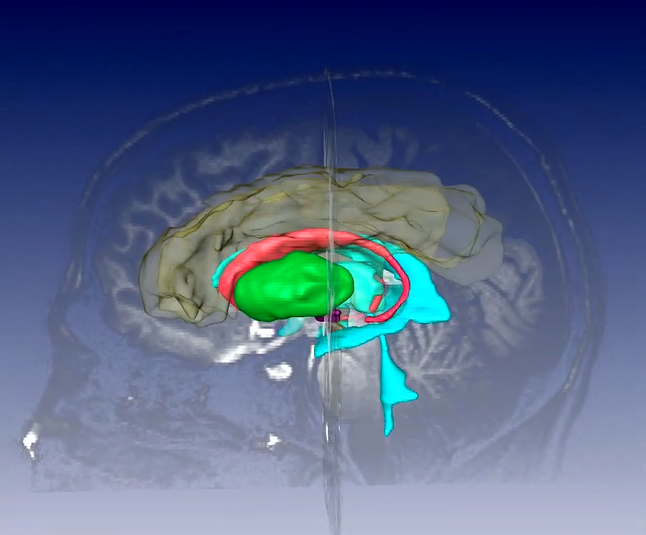
\includegraphics[width=0.8\linewidth]{BG_3D_screenshot}
			\captionof{figure}{3D Reconstruction\\
				of the BG \parencite{BG}}
		\end{minipage}
		\hfill
	\end{adjustbox}
}

\headerbox{Overview}{name=overview,column=2,row=0, span=4}{
	\begin{adjustbox}{minipage=0.95\textwidth, margin=5pt, center}
		\begin{minipage}[r]{0.65\textwidth}
			\justifying
				\textbf{Task:}
				We have implemented a virtual iCub robot in the plane that is able to link proprioceptive information with a target coordinate \textcolor{red}{target position} (Figure 2). It links both the initial proprioceptive information of the \textcolor{blue}{initial position} and the proprioceptive information of the \textcolor{blue}{target position}\\[3pt]
				\textbf{Training:}Like in Baladron et al. \parencite{baladronContributionBasalGanglia2023b} through infantile motor babbling, our network forms associations between the action (changed joint angle) and the outcome (position of the changed joint angle). The initial state (initial joint angle) is projected into the striatum via the S1, which makes it possible to learn the proprioceptive context under different \textcolor{blue}{initial positions}.\\[3pt]
				\textbf{Features:}
				Shows how motor learning of proprioceptive context occurs via CBGT-loops with possible implications of a more dynamical role of the BG in both action selection and movement modulation \parencite{parkBasalGangliaCircuits2020}
		\end{minipage}
		\hfill
		\begin{minipage}[r]{0.3\textwidth}
			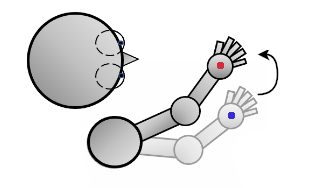
\includegraphics[width=\linewidth]{movement_plan}
			\captionof{figure}{Virtual iCub environment}
		\end{minipage}
		\hfill
	\end{adjustbox}
}


\headerbox{Computational Model}{name=model, column=0, below=infos, span=2}{
	\begin{adjustbox}{minipage=0.95\textwidth, margin=5pt, center}
		\begin{minipage}[t]{\textwidth}
			\centering
			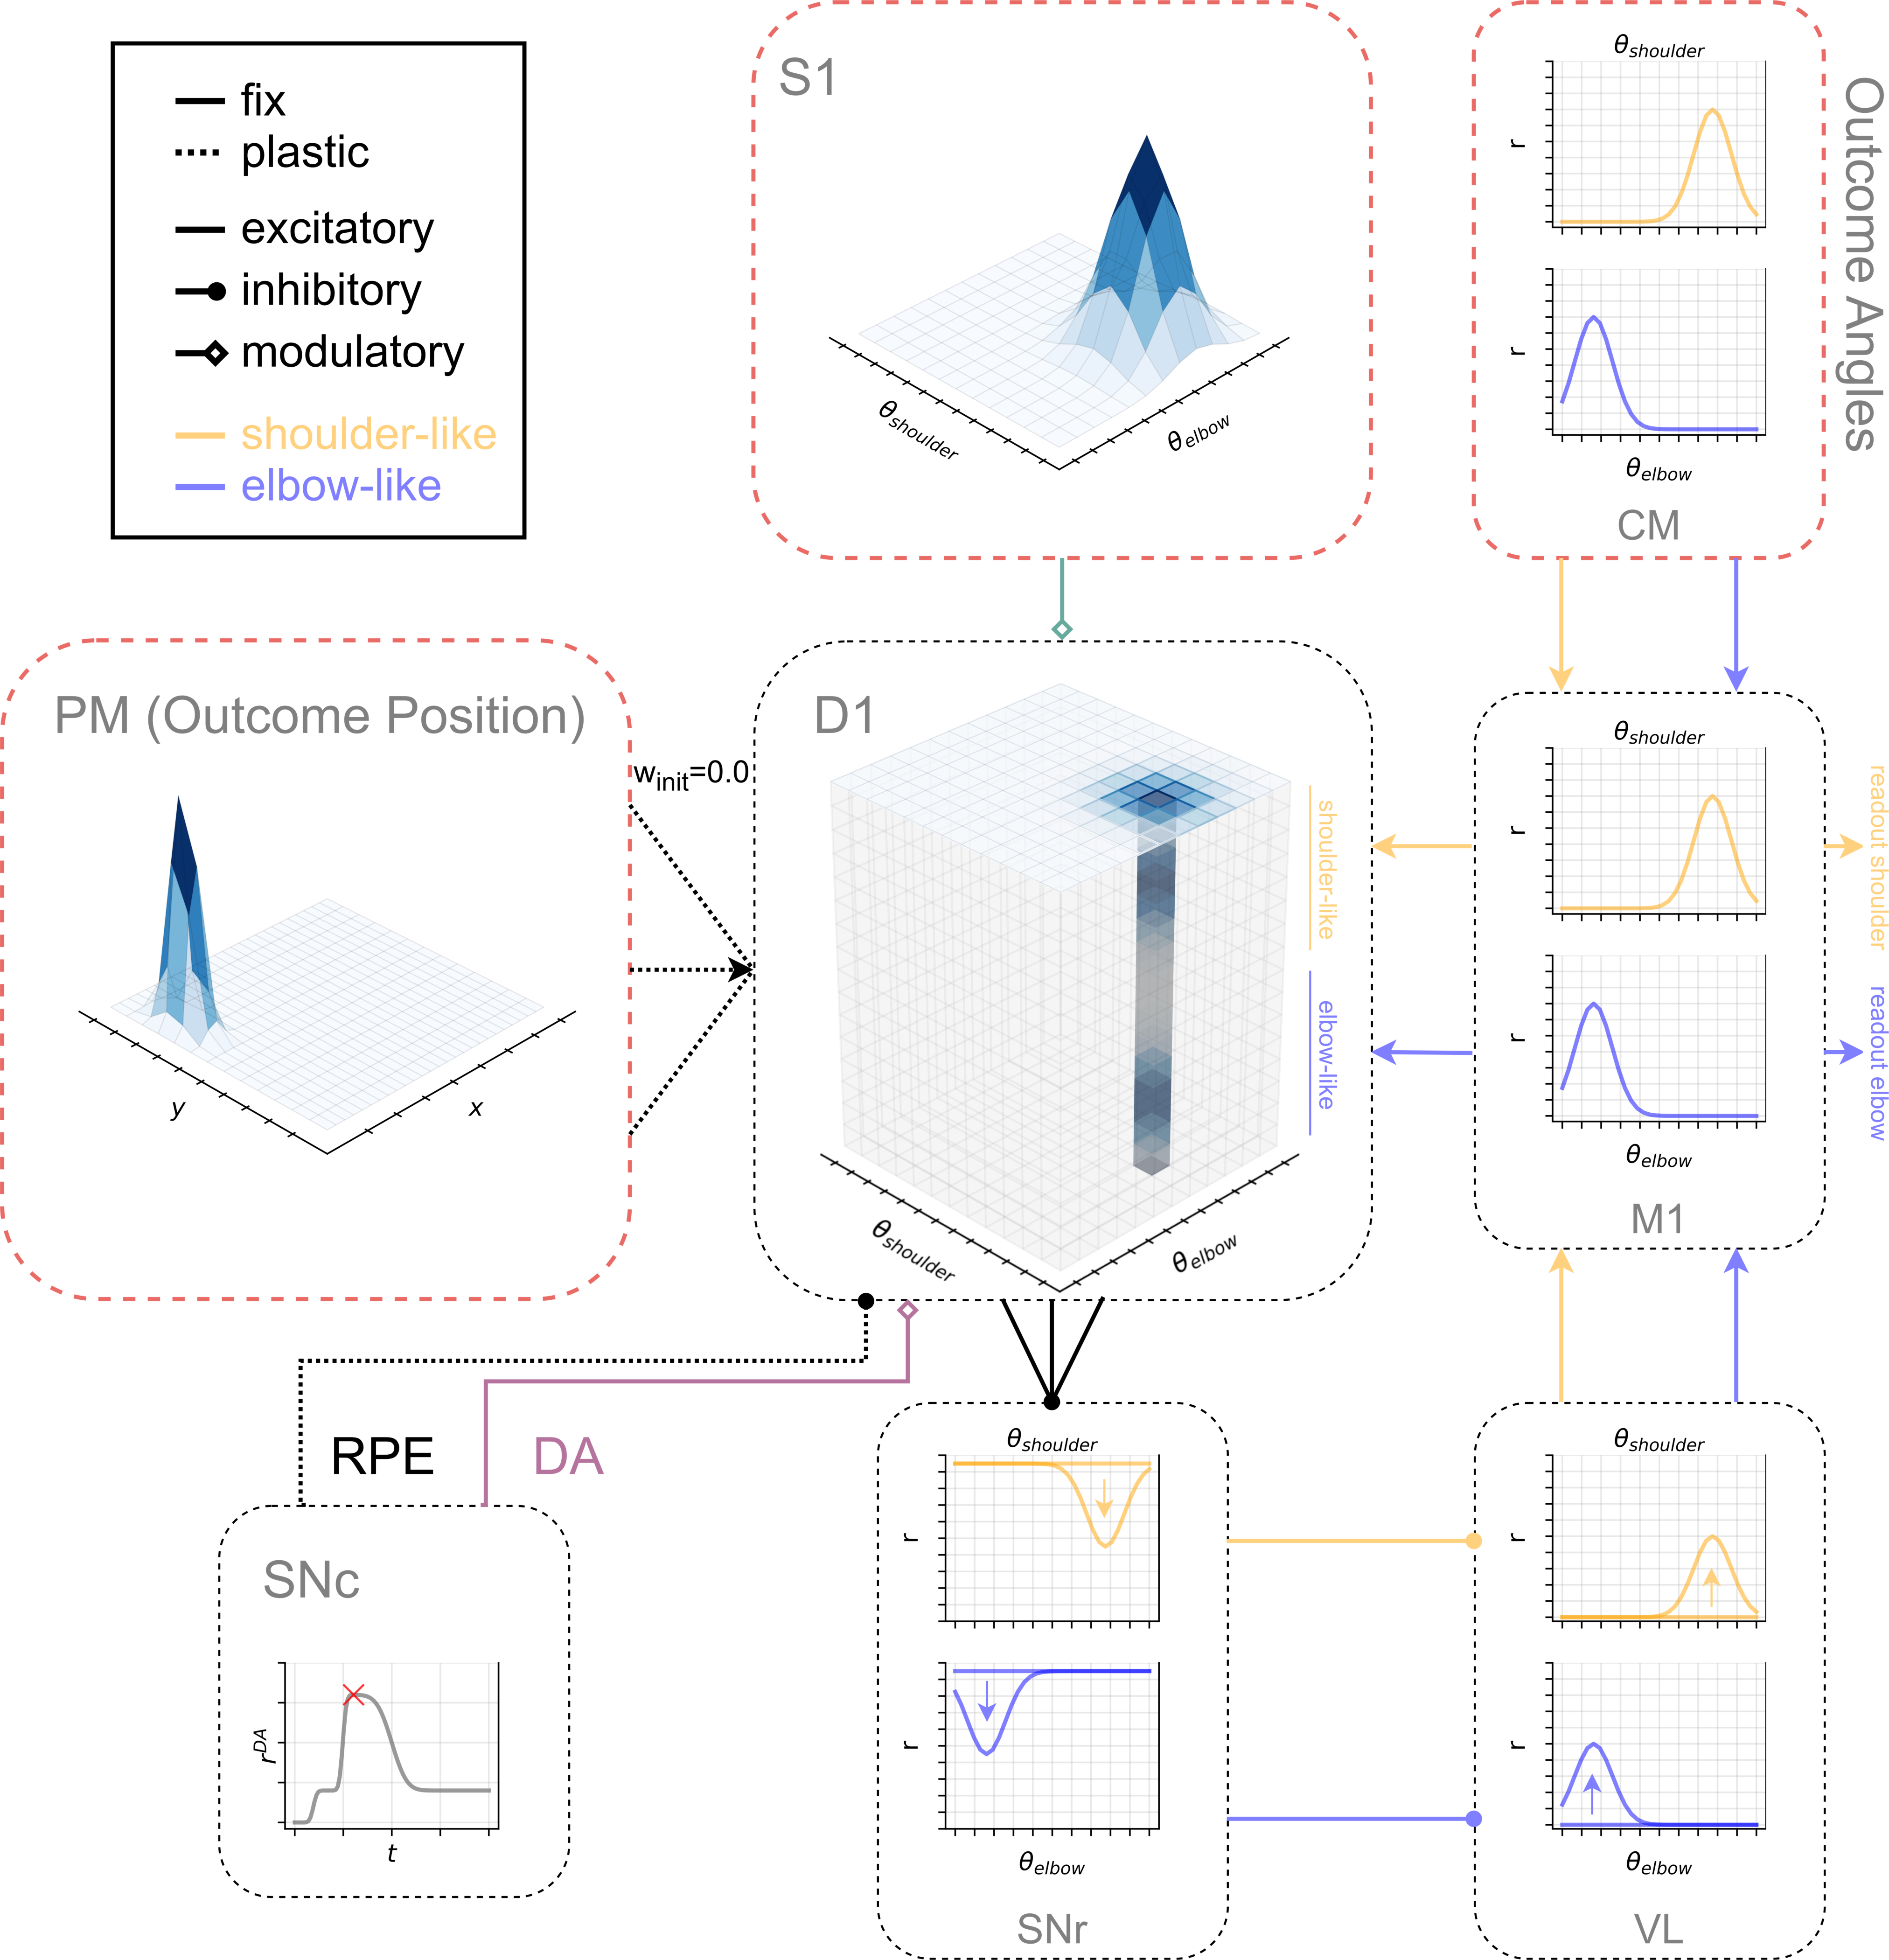
\includegraphics[width=\linewidth]{model}
			\captionof{figure}{Overview of the model}
			\vspace{5pt}
		\end{minipage}
		\hfill
		\begin{minipage}[b]{\textwidth}
			\justifying
\textbf{\textcolor{training-set}{Input Populations}}:\\[4pt]
\footnotesize
\textbf{PM}: Encodes the target position in the reaching space. A 3-factor learning rule is used to establish connections to active D1 patches (see Model definitions).\\[2pt]
\textbf{S1}: Encodes current joint angles via gain fields. S1 sends projections that diverge to innervate multiple regions in the Striatum (D1 patches) \parencite{flahertyCorticostriatalTransformationsPrimate1991}\\[2pt]
\textbf{CM}: Centro median nuclei located in the intralaminar nuclei sends proprioceptive information of the target position into the M1. This connection is deactivated in the test phase.\\[10pt]
\small
\textbf{Recurrent Populations:}\\[4pt]
\footnotesize
\textbf{D1} (Striatum): Activity in S1 and M1 activates certain patches of D1 receptors in the striatum\\[2pt]
\textbf{SNr}: Pooling takes place from D1 $\rightarrow$ SNr. Active joint angle encodings in D1 inhibit corresponding neurons in SNr\\[2pt]
\textbf{VL}: Inactive SNr neurons disinhibit VL neurons\\[2pt]
\textbf{M1}: M1 encodes shoulder like and elbow like neurons via population code 
\parencite{pruszynskiPrimaryMotorCortex2011}, which map the joint angle to a specific coordinate. The weighted sum of the M1 activity is the angle of the corresponding joint\\[2pt]
\textbf{SNc}: Dopamine (DA) is released through movement \parencite{cheungLearningCriticallyDrives2023}, which makes the connections between PM $\rightarrow$ D1 plastic. Active D1 neurons inhibit DA release (\textit{RPE})

		\end{minipage}
	\end{adjustbox}
}


\headerbox{Model Definitions}{name=definitions, column=2, below=overview, span=4}{
	\begin{adjustbox}{minipage=0.95\textwidth, margin=5pt, center}
		\begin{minipage}[r]{0.475\textwidth}
			\justifying
		The model is implemented in Python 3.12 with the neurosimulator ANNarchy 4.7.3 \parencite{vitayANNarchyCodeGeneration2015}. All neurons are rate-coded.\\
				
		\textbf{Neuron model:}\\
		$$
		\tau \frac{d r^{post}_j }{ dt } + r^{post}_j = \sum_{i \in exc}{w_{ij} \cdot r^{pre}_i} - \sum_{i \in inh}{w_{ij} \cdot r^{pre}_i} + baseline + \xi 
		$$
		$${mp}(t) = \begin{cases}\operatorname{logistic}{\left({r}(t) \right)}\qquad \text{if} \quad {r}(t) > 1.0\\ ({r}(t))^+ \qquad \text{otherwise.} \end{cases} \hspace{2em} \text{with:  } \xi \sim \mathcal{U}$$
		
		
		\textbf{Synaptic learning rules:}\\
		$$\tau_w \frac{d w_{ij} }{ dt } = m_{DA} \cdot C_{ij} - \alpha \left(r^{post}_j - \bar{r}^{post} - \gamma^{post}\right)^2$$
		\end{minipage}
		\hfill
		\begin{minipage}[r]{0.475\textwidth}
		\justifying
		$$m_{DA} = const \cdot \left(r^{DA} - baseline_{DA}\right) \hspace{1.5em} \tau_{\alpha} \frac{d \alpha_j }{ dt } + \alpha_j = (r^{post}_j - \Theta)$$
		\textit{Cortico-striatal} (PM $\rightarrow$ D1)
		$$ C_{ij} = \left(r^{pre}_j - \bar{r}^{pre} - \gamma^{pre}\right)^+ \left(r^{post}_j - \bar{r}^{post} - \gamma^{post}\right) $$	
		\textit{Reward Prediction Error (RPE):} (D1 $\rightarrow$ SNc)\\[3pt]
			When certain´ D1 neurons are repeatedly active, they inhibit the DA release ($r^{DA}$) in the SNc. 
			This prevents new associations from being learned by the same striatum neurons (\textit{novelty learning}).\\
			$$ \tau \frac{d w_{j}^{DA}}{dt} =  \left(r^{DA} - baseline_{DA}\right)^+ \left( r^{pre}_j - \bar{r}^{pre} - \gamma^{pre}\right)^+ $$
		\end{minipage}
	\end{adjustbox}
}

\headerbox{References}{name=refs, column=0, above=bottom, span=5}{
	\begin{adjustbox}{minipage=0.975\textwidth, margin=0pt, center}
		\compressbib{\printbibliography[heading=none]}
	\end{adjustbox}	
}

\headerbox{Results}{name=res, column=2, below=definitions, above=refs, span=4}{
	\begin{adjustbox}{minipage=0.95\textwidth, margin=5pt, center}
		\begin{minipage}[t]{0.475\textwidth}
			\textbf{Reaching:}\\[2pt]
			A random \textcolor{red}{target position} is activated in the PM. If the association was learned during training, certain D1 patches become active and disinhibit the VL. M1 becomes active. \\[10pt]
		\begin{center}
			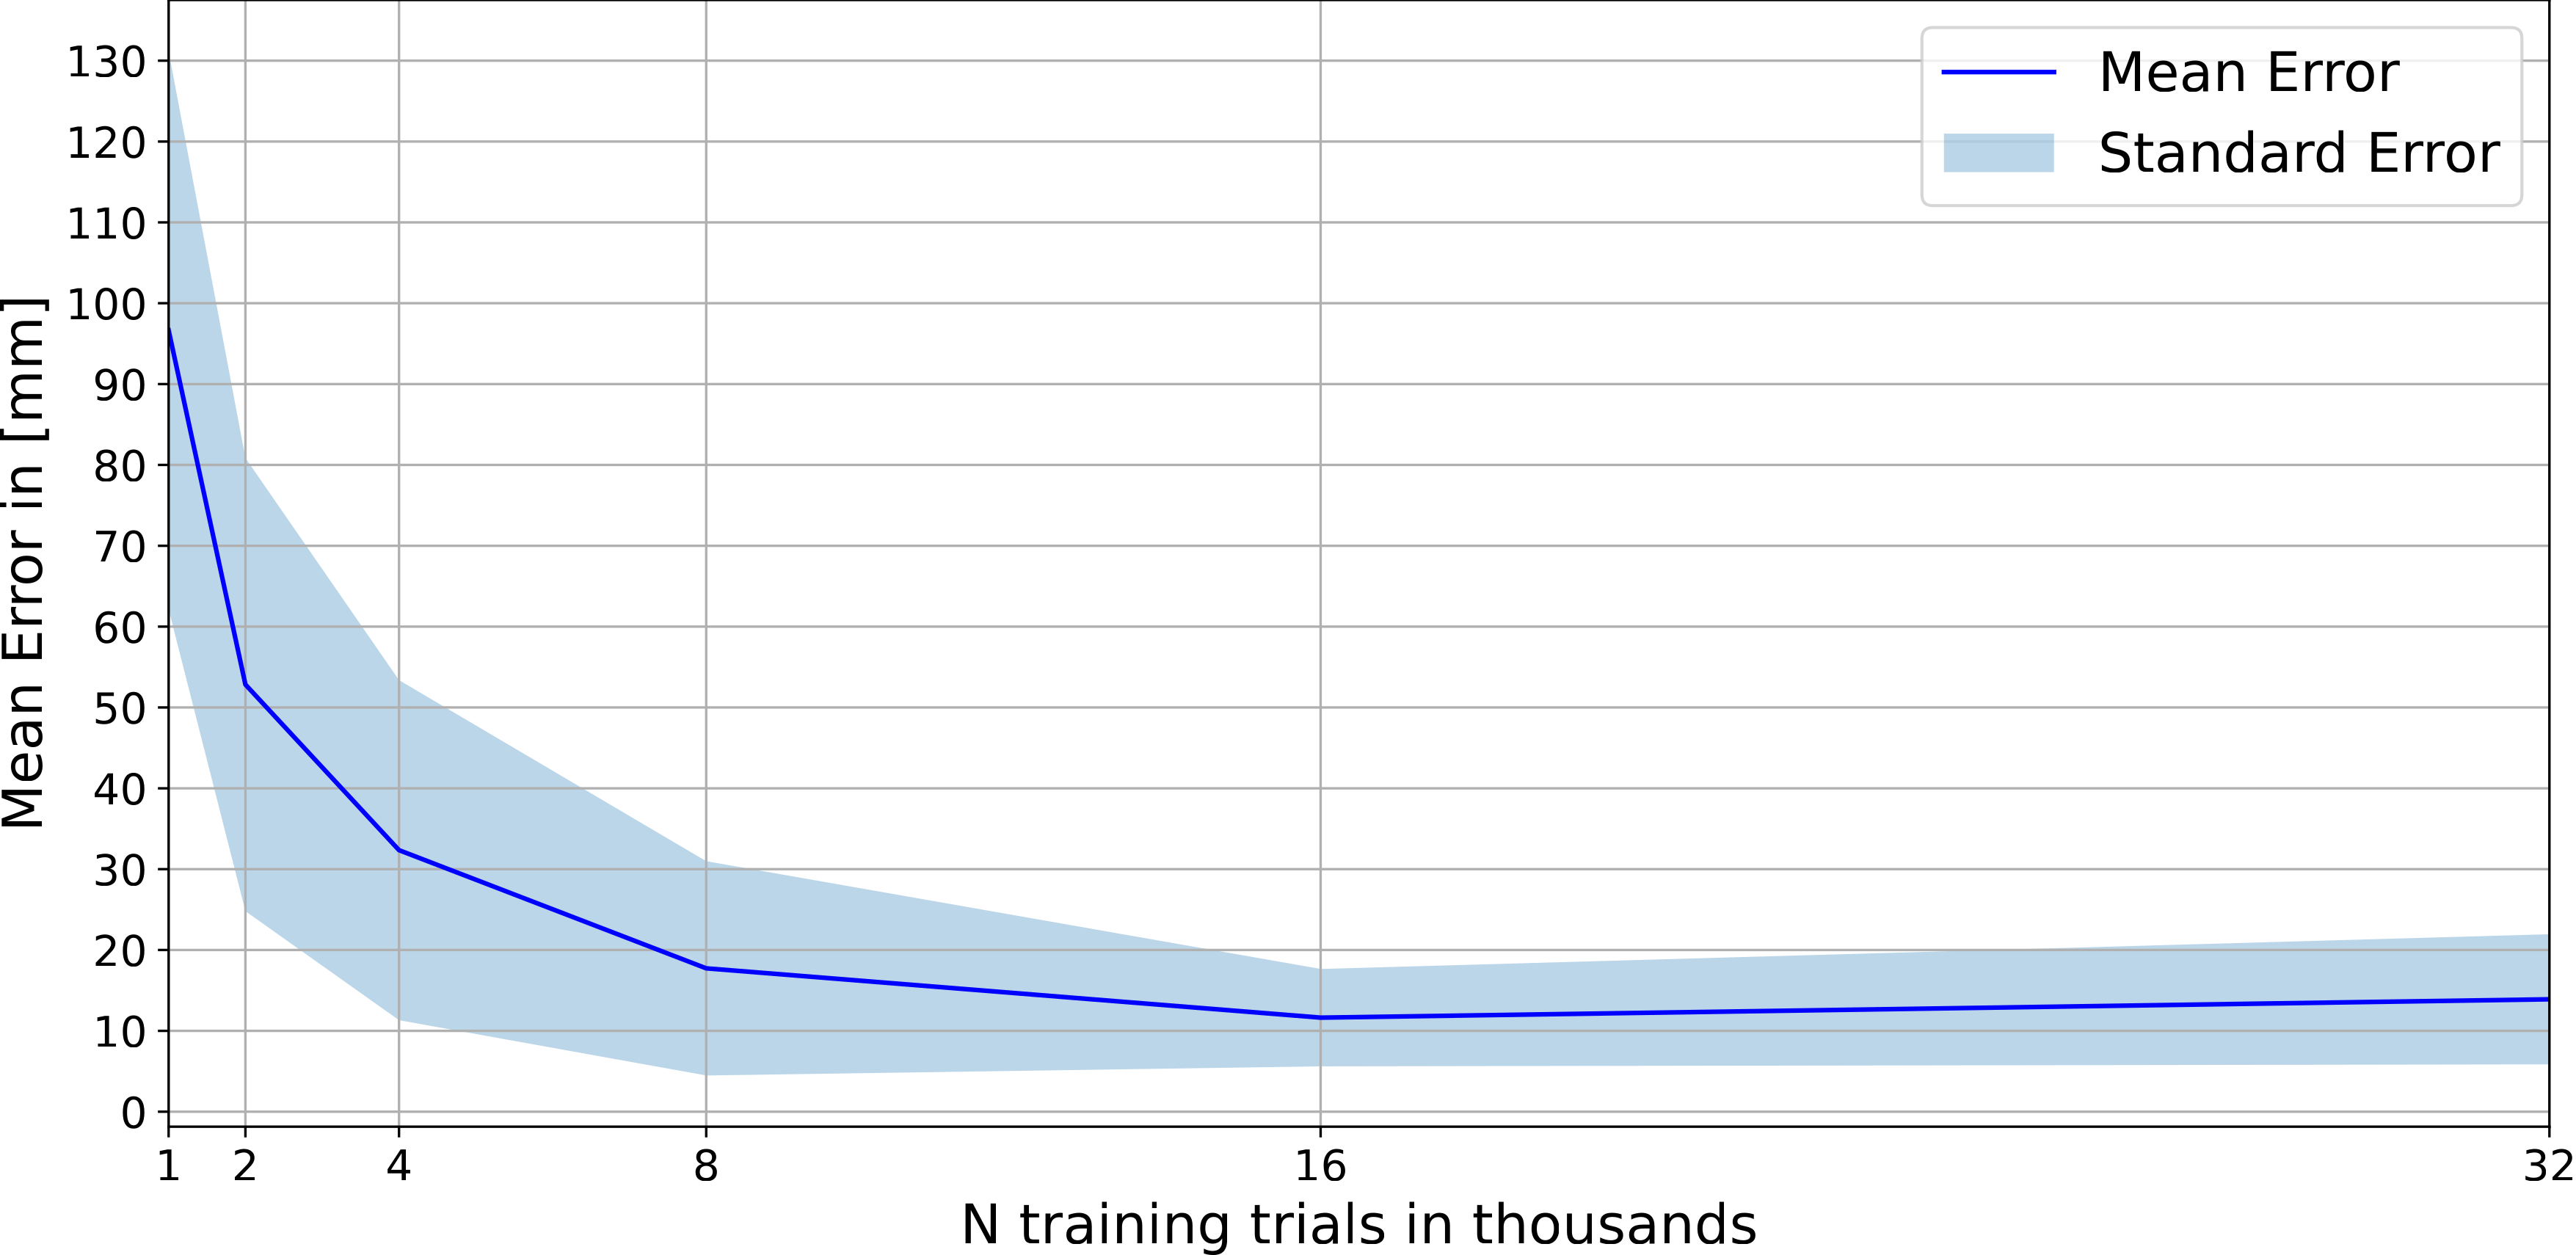
\includegraphics[width=\linewidth]{bg_error_plot}
			\captionof{figure}{Mean Error in the reaching task}
		\end{center}
		\end{minipage}
		\hfill
		\begin{minipage}[t]{0.475\textwidth}
			\textbf{Perturbation:}\\[2pt]
			A random \textcolor{red}{target position} is activated in the PM. As the activities build up, the joint angles in S1 are perturbed by a random amount by $\Delta \theta_{shoulder}$ and $\Delta \theta_{elbow}$. Both drawn from a Uniform Distribution $\mathcal{U}[-10^\circ, 10^\circ]$.\\
			\begin{center}
				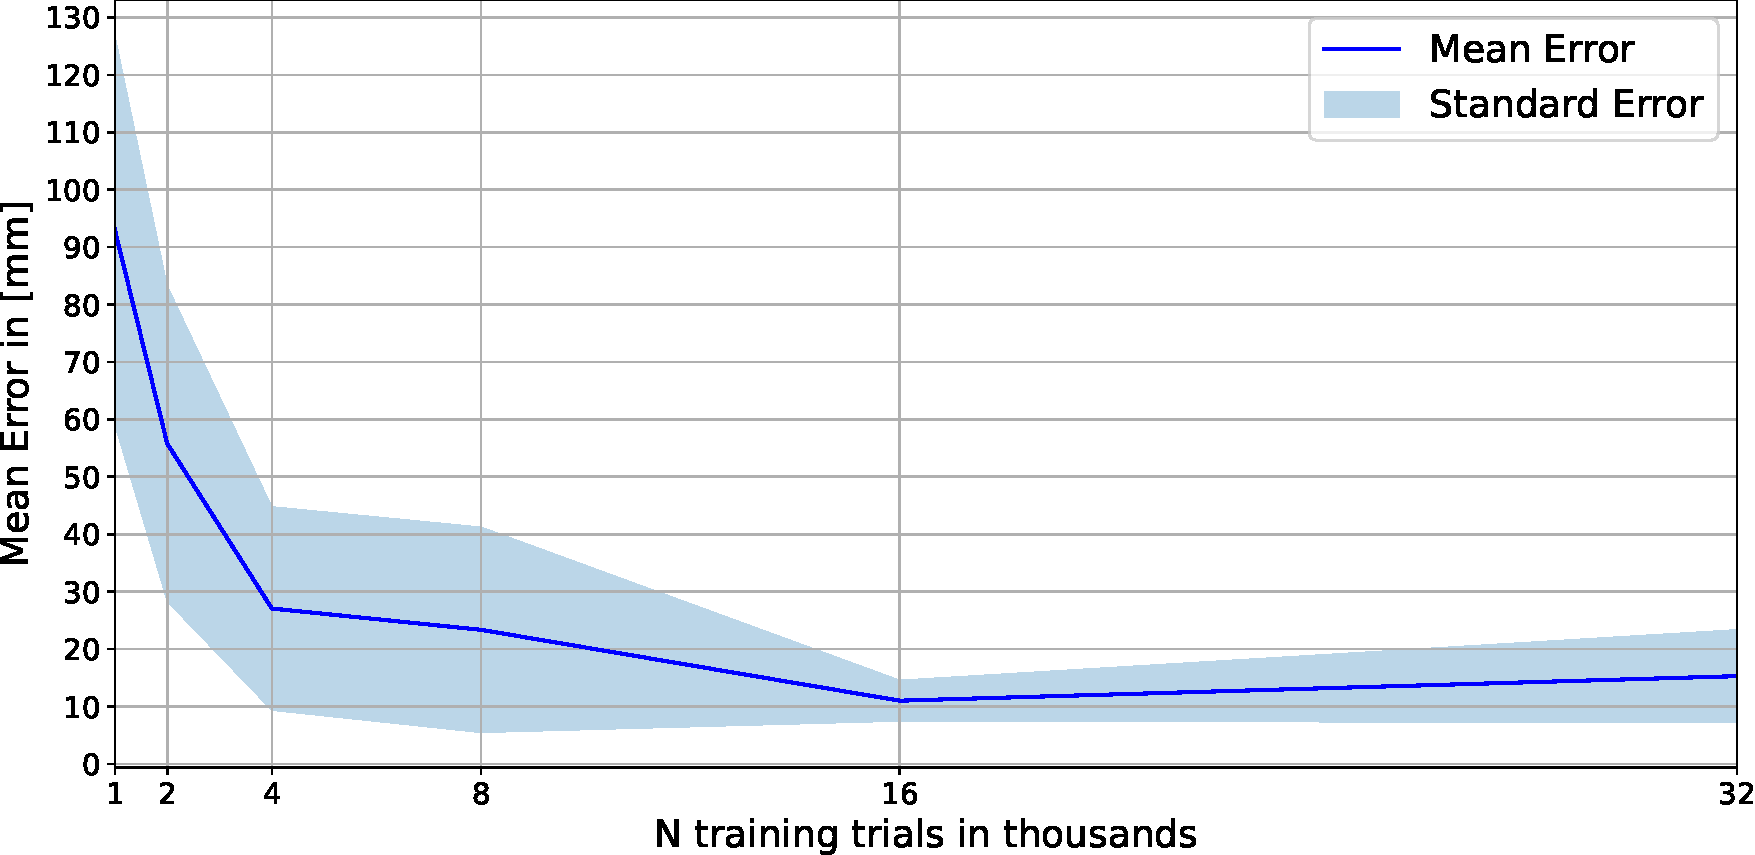
\includegraphics[width=\linewidth]{bg_error_plot_perturbation}
				\captionof{figure}{Mean Error in the perturbation task}
			\end{center}
		\end{minipage}
		\hfill
		\begin{minipage}[t]{0.25\textwidth}
			\vspace{8pt}
			\textbf{Modulation of the population code:}\\[2pt]
			A random \textcolor{red}{target position} was learned. Figure 6 shows the population code of shoulder-like and elbow-like neurons under different scaling in D1. The activity of the D1 neurons has a direct influence on the norm of the population code \parencite{parkBasalGangliaCircuits2020}.\\
			\begin{center}
				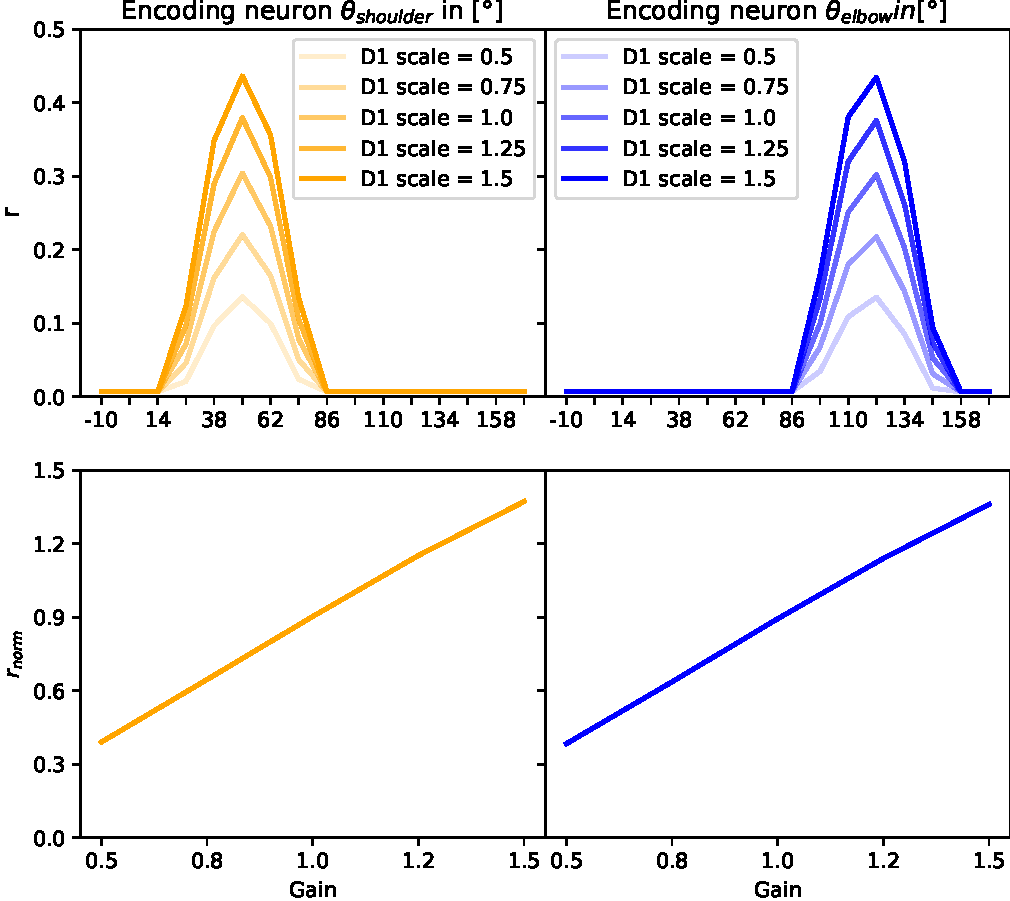
\includegraphics[width=1.1\linewidth]{d1_gain}
				\captionof{figure}{After 100 ms simulation}
			\end{center}
		\end{minipage}
		\hfill
		\begin{minipage}[t]{0.725\textwidth}
			\vspace{8pt}
			\textbf{Comparison to Deep RL methods:}\\[2pt]
			In order to solve the reaching task with a \textit{PPO} \parencite{schulmanProximalPolicyOptimization2017} and a \textit{TD3} Agent \parencite{fujimoto2018addressing} the problem is formalised as a MDP with state $s$ and possible actions $a$:\\[-8pt]
			\begin{center}
				$s = [\sin(\underline{\theta}),  \cos(\underline{\theta}), \underline{x}_{error}] \hspace{10pt} a = \Delta\underline{\theta}\hspace{10pt} \text{with:  } \underline{\theta}=\begin{bmatrix}
					\theta_{shoulder} \\
					\theta_{elbow} \\ 
				\end{bmatrix} \hspace{10pt} 
				\underline{x}_{error}=\begin{bmatrix}
					\left\lVert x_{target} - x_{current} \right\rVert \\
					\left\lVert y_{target} - y_{current} \right\rVert \\ 
				\end{bmatrix}  \vspace{5pt}
				$
			\end{center}
			The reward $r$ is defined as the negative L2 norm between current and target position (dense reward setting). In addition, there is a sparse positive reward if an action is close enough to the target position, or a sparse negative reward if an action leads outside the joint constraints.\\[5pt]
			\begin{center}
				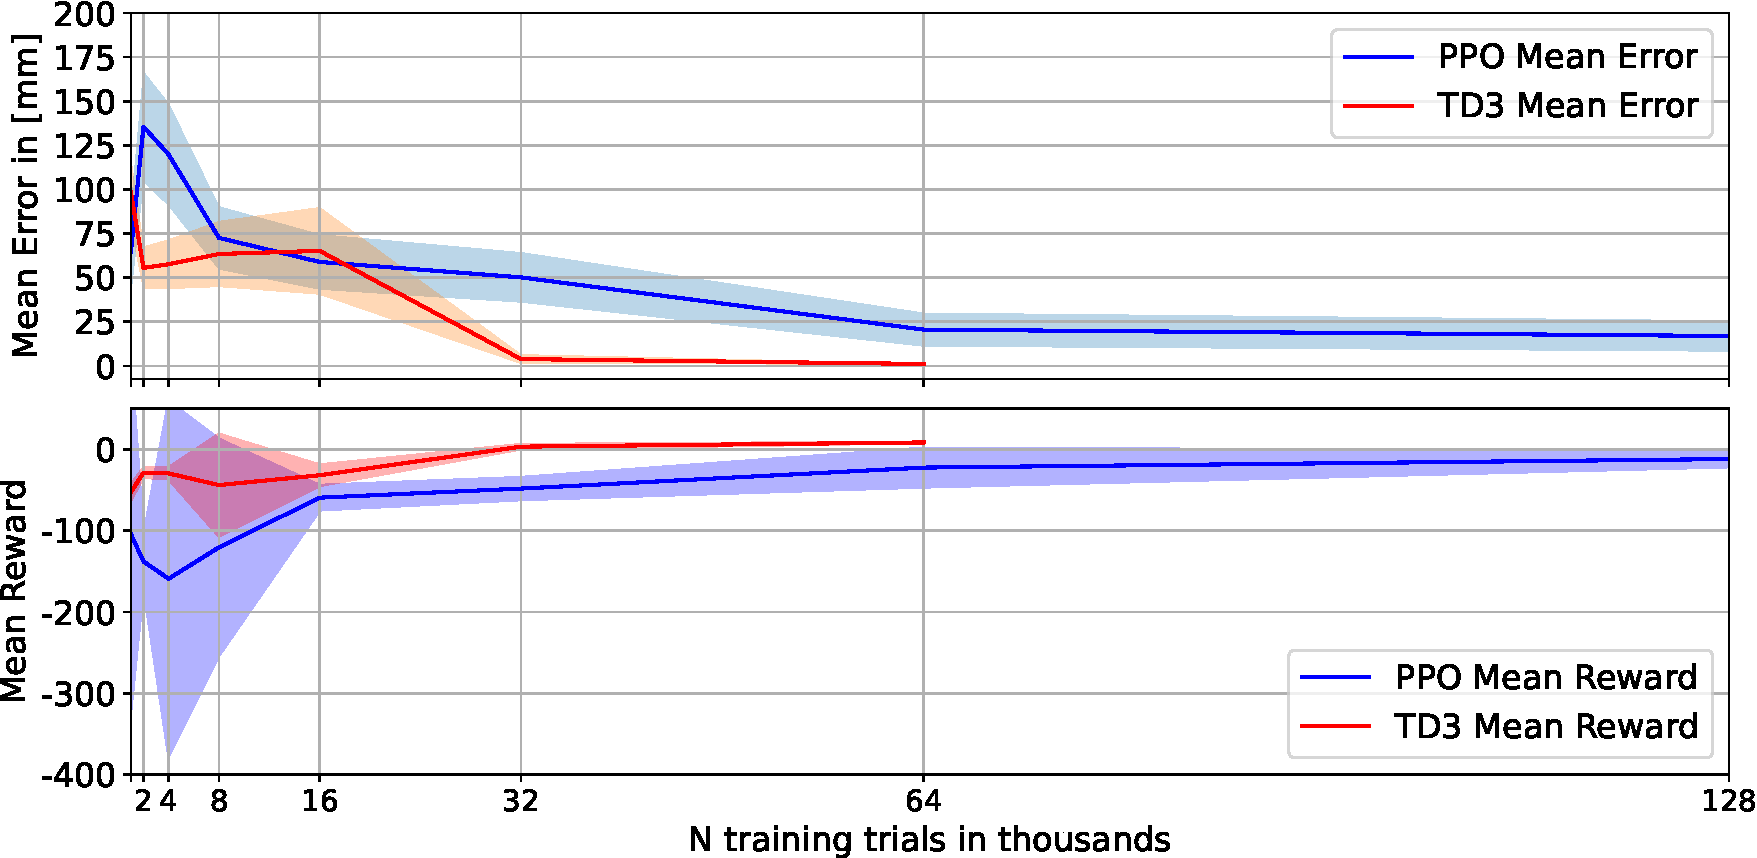
\includegraphics[width=0.8\linewidth]{drl_error_plot}
				\captionof{figure}{Performance of the \textit{PPO} and \textit{TD3} trained Network}
			\end{center}
		\end{minipage}
		\hfill
	\end{adjustbox}

}


\headerbox{Procedure}{name=res, column=0, below=model, above=refs , span=2}{
	\begin{adjustbox}{minipage=0.95\textwidth, margin=5pt, center}
		
		\begin{minipage}[t]{\textwidth}
			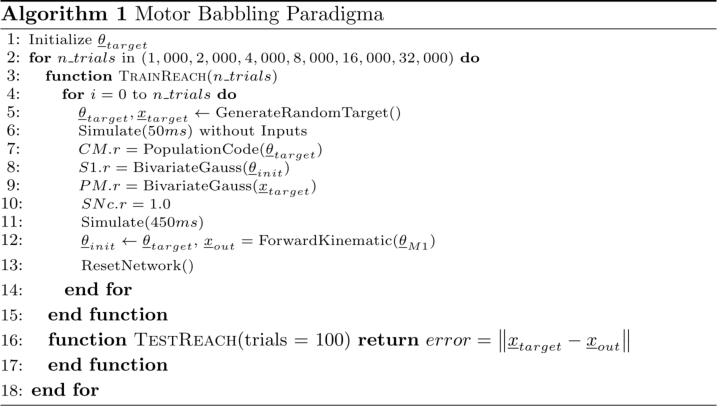
\includegraphics[width=0.95\textwidth]{training}	
		\end{minipage}
		
	\end{adjustbox}	
}


\headerbox{\large Acknowlegdements}{name=ack, column=5, above=bottom, below=res, span=1}{	
	\begin{adjustbox}{minipage=0.925\textwidth, margin=5pt, center}
	\vfill
	This work was supported by the DFG priority program ”The Active Self” 
	HA2630/12-2.\\[2pt]
	\begin{center}
		\textit{Repository:}\\[2pt]
		
\includegraphics[width=\linewidth]{githubQR}
	\end{center}
		
	\end{adjustbox}
}


\end{poster}


\end{document}